
\begin{figure}[H]
    \centering
    \begin{subfigure}[b,height=2cm]{0.22\textwidth}
         \centering
         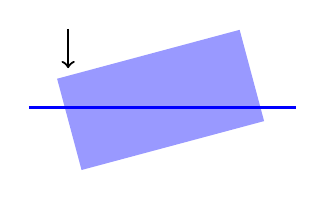
\begin{tikzpicture}

            \fill [blue!40, rotate around={15:(0,0.0)}] (-1.2,-0.5) rectangle (1.2,0.7);
            \draw[blue, thick] (-1.7,0) -- (1.7,0);
            \draw[black, thick, ->] (-1.2,1) -- (-1.2,0.5);
          
          \end{tikzpicture}
         \caption{The ship model is forces to an initial angle and then released}
         \label{fig:rolldecay_initial}
     \end{subfigure}
     \hfill
     \begin{subfigure}[b,height=2cm]{0.22\textwidth}
         \centering
         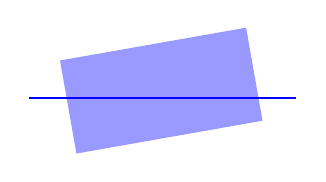
\begin{tikzpicture}

            \fill [blue!40, rotate around={10:(0,0.0)}] (-1.2,-0.5) rectangle (1.2,0.7);
            \draw[blue, thick] (-1.7,0) -- (1.7,0);
            
          \end{tikzpicture}
         \caption{Starts to roll back}
         \label{fig:rolldecay_free}
     \end{subfigure}
     \hfill
     \begin{subfigure}[b,height=2cm]{0.22\textwidth}
         \centering
         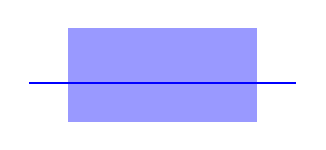
\begin{tikzpicture}

            \fill [blue!40, rotate around={0:(0,0.0)}] (-1.2,-0.5) rectangle (1.2,0.7);
            \draw[blue, thick] (-1.7,0) -- (1.7,0);
            
          \end{tikzpicture}
         \caption{Static equilibrium}
         \label{fig:rolldecay_equilibrium}
     \end{subfigure}
    \hfill
     \begin{subfigure}[b,height=2cm]{0.22\textwidth}
         \centering
         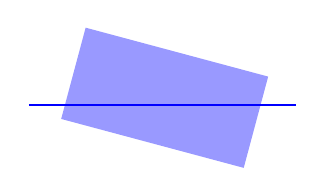
\begin{tikzpicture}

            \fill [blue!40, rotate around={-15:(0,0.0)}] (-1.2,-0.5) rectangle (1.2,0.7);
            \draw[blue, thick] (-1.7,0) -- (1.7,0);
            
          \end{tikzpicture}
         \caption{End point other side}
         \label{fig:rolldecay_endpoint}
     \end{subfigure}
    \caption{Roll decay test.}
    \label{fig:rolldecay_procedure}
\end{figure}